\chapter{5-coloring of planar graphs}

Write the following recirsive algorithm for 5-coloring of planar graphs:

\medskip
\noindent Find a vertex $x$ of minimum degree.
\begin{enumerate}
    \item if the vertex $x$ is of degree 4 or less, remove it, color the smaller graph and extend the coloring to $x$,
    \item f the vertex $x$ is of degree 5 remove it, identify two non-adjacent neighbors $u$ and $v$ of $x$, color the smaller graph and extend the coloring to $x$. Note: if the neighbors of $x$ in the \textbf{embedding} are $x_0$, $x_1$, $x_2$, $x_3$, $x_4$ then either we take $u$ = $x_0$ and $v$ = $x_2$, if $x_0$ and $x_2$ are not adjacent, or $u$ = $x_1$ and $v$ = $x_3$, otherwise.
\end{enumerate}

\medskip
\noindent \textbf{Note:}
Use the following built-in Sage methods on graphs:
\begin{itemize}
\item \verb|G.is_planar(set_embedding=True, set_pos=True)| checks for planarity and, optionally, sets coordinates and combinatorial embedding (clockwise ordering of neighbors at each vertex)
\item  Subsequent call to the method \verb|G.faces()| returs the faces of the graph (as lists of edges) and a call to the method \verb|G.get_embedding()| returns the combinatorial embedding (mapping from vertices to lists of neighbors in clockwise order around the vertex).
\item  \verb|G.plot()| plots the graph with the given embedding and coordinates (if it is planar).
\end{itemize}

\medskip
Example:
\begin{sageCell}
    H = Graph({0:[1,2,3], 1:[4,5], 2:[6], 3:[4,6], 4:[7], 5:[7], 6:[7]})
    H.is_planar(set_embedding=True, set_pos=True)
\end{sageCell}
\begin{outCell}
    True
\end{outCell}

\begin{sageCell}
    H.plot()
\end{sageCell}
\begin{outImage}
   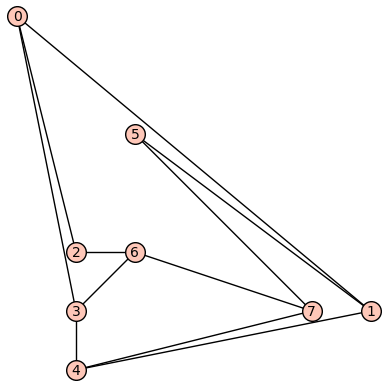
\includegraphics[width=0.6\textwidth]{Images/5-coloring/planar_graph.png}
\end{outImage}

\begin{sageCell}
    H.faces()
\end{sageCell}
\begin{outCell}
    [[(0, 1), (1, 4), (4, 3), (3, 0)],
     [(0, 2), (2, 6), (6, 7), (7, 5), (5, 1), (1, 0)],
     [(0, 3), (3, 6), (6, 2), (2, 0)],
     [(1, 5), (5, 7), (7, 4), (4, 1)],
     [(3, 4), (4, 7), (7, 6), (6, 3)]]
\end{outCell}

\begin{sageCell}
    H.get_embedding()
\end{sageCell}
\begin{outCell}
    {0: [1, 2, 3],
     1: [4, 5, 0],
     2: [0, 6],
     3: [0, 6, 4],
     4: [3, 7, 1],
     5: [1, 7],
     6: [2, 7, 3],
     7: [5, 4, 6]}
\end{outCell}

\section{Solution}

\begin{sageCell}
def color_planar_5(G):
    if not G.is_planar(set_embedding=True):
        raise Exception("Input is not a planar graph.")
    emb = G.get_embedding()

    return color_planar_5_rec(emb)
\end{sageCell}

\begin{sageCell}
def color_planar_5_rec(emb):
    # Graph has <= 5 vertices
    if len(emb) <= 5:
        vertices = emb.keys()
        col = dict(zip(vertices, [0, 1, 2, 3, 4]))
        return col

    # Find vertex with min degree
    x = min(emb, key = lambda v: len(emb[v]))

    if len(emb[x]) < 5:
        return color_planar_5_d4(emb, x)
    else:
        return color_planar_5_d5(emb, x)

def color_planar_5_d4(emb, x):

    # remove x from the graph
    Nx = emb[x]
    for w in Nx:
        emb[w].remove(x)
    del emb[x]

    # color the rest
    col = color_planar_5_rec(emb)

    # extend to x
    used = [col[w] for w in Nx]
    free = [c for c in [0, 1, 2, 3, 4] if c not in used]
    col[x] = free[0]

    return col

def color_planar_5_d5(emb, x):

    # choose u,v to identify
    Nx = emb[x]
    if Nx[0] in emb[Nx[2]]:
        u,v = Nx[1], Nx[3]
    else:
        u,v = Nx[0], Nx[2]

    # u and v have a common neighbor x,
    # for other common neighbors w we remove
    # the edge wu (no double edges!)
    for w in emb[v]:
        if w != x and w in emb[u]:
            emb[u].remove(w)
            emb[w].remove(u)

    # identify u and v
    ux = emb[u].index(x)
    vx = emb[v].index(x)
    emb[u] = emb[u][:ux] + emb[v][vx + 1:] + emb[v][:vx] + emb[u][ux + 1:]
    for w in emb[v]:
        wv = emb[w].index(v)
        emb[w][wv] = u
    del emb[v]

    # remove the vertex x
    for w in Nx:
        if w != u and w != v:
            emb[w].remove(x)
    del emb[x]

    # color the rest
    col = color_planar_5_rec(emb)

    # extend the coloring
    used = [col[w] for w in Nx if w in col]
    free = [c for c in [0, 1, 2, 3, 4] if c not in used]
    col[v] = col[u]
    col[x] = free[0]

    return col
\end{sageCell}


